% ----------------------------------------------------------
\chapter{Fundamentação Teórica}\label{cap:fundamentacaoTeorica}
% ----------------------------------------------------------
Explicar brevemente o que será tratado como fundamentação teórica para o entendimento do contexto em que o modelo de aprendizagem de máquina será aplicado.

\section{As mudanças climáticas e as catástrofes naturais}

As grandes cidades brasileiras enfrentam desafios mais frequentes relacionados às mudanças climáticas, que agravam problemas como enchentes, inundações e deslizamentos. Projeções indicam que, até 2030, a mancha urbana de São Paulo pode aumentar em até 38\%, ampliando o risco para mais de 20\% das áreas de expansão urbana, que se tornarão suscetíveis a acidentes naturais (Nobre et al., 2011). O estudo também destaca que o aumento na frequência de eventos de chuvas intensas pode dobrar o número de dias com precipitação acima de 10 milímetros, agravando a vulnerabilidade da população, especialmente nas áreas periféricas e de menor infraestrutura.

\subsection{Cenário de enchentes no sul do Brasil}

Com base no histórico das enchentes no Rio Grande do Sul, observa-se que os desastres relacionados ao excesso de chuvas não são um fenômeno recente. Desde 1941, o estado lida com eventos catastróficos, como a enchente que devastou Porto Alegre naquele ano, considerada uma das mais graves da história da cidade. Ao longo das décadas, esses episódios continuaram a ocorrer, expondo a vulnerabilidade da região diante de chuvas intensas e repentinas. A combinação de fatores naturais, como a geografia da região e os ciclos climáticos, aliado as ações humanas nocivas ao meio ambiente, contribui para a repetição e intensificação dessas tragédias \cite{veja2024}.

Em Santa Catarina, estado adjacente ao Rio Grande do Sul, as enchentes também são fenômenos recorrentes que, ao longo dos anos, têm causado impactos sociais, econômicos e ambientais. Um dos eventos mais recentes foi registrado em maio de 2024, quando o estado registrou vários dias com altos indíces pluviométricos, levando ao transbordamento de rios, deslizamentos de terra e bloqueios em diversas rodovias \cite{g12024}.

\subsection{Dinâmica do Rio Guaíba}

O Rio Guaíba, principal manancial de abastecimento de água para a capital do Rio Grande do Sul e região, é alvo de estudo sobre diversos temas, incluindo sua hidrodinâmica e nível ao longo do ano. No Artigo conduzido pelos pesquisadores \cite{andrade2017}, a variabilidade nas descargas líquidas do Rio Guaíba revelou flutuações significativas nos volumes de descarga, variando de 407 m³/s a 14.270 m³/s, o que indica uma grande influência das condições climáticas sazonais e da vazão dos rios tributários, como o Jacuí, Taquarí, Caí e Sinos. Essas variações extremas foram observadas durante o período de 2014 a 2017 e reforçam a importância de monitorar continuamente o regime de águas do Guaíba para prevenir enchentes e outros desastres associados \cite{andrade2017}.

\section{Aprendizado de máquina}

Desde que os computadores foram inventados, criou-se o questionamento da possibilidade de fazê-los pensar de modo semelhante ao ser humano. Por meio desse avanço, diversas áreas sofreriam grandes transformações, uma vez que a capacidade da máquina aprender e aprimorar o seu conhecimento sobre determinado assunto traria melhorias e uma maior performance na atividade desejada \cite{carbonell1983}.

Embora os computadores ainda não alcancem o mesmo nível de aprendizado geral do ser humano, nos últimos anos, o aprendizado de máquina (do inglês, \textit{machine learning}, ou ML) se tornou realidade, com aplicações em diversos setores relacionados ou não a tecnologia, agregando valor e conhecimento por meio de dados e informações antes tratados apenas por profissionais da área.

Esse conceito envolve a criação de sistemas que são capazes de aprender a partir de dados, identificando padrões e realizando previsões sem a necessidade de programação explícita. De acordo com \cite{carbonell1983}, o principal objetivo do ML é construir algoritmos que permitam que os computadores adquiram conhecimento e melhorem sua performance de forma autônoma, baseando-se em experiências passadas.

\subsection{Categorias de aprendizado de máquina}

Com pesquisas e algoritmos sendo desenvolvidos para novas aplicações e/ou aprimoramento de implementações existentes, tornou-se necessário criar categorias de ML, a fim de classificar a sua função e estipular em quais cenários o seu uso é adequado.

Os quatro principais tipos de ML são: supervisionado, não supervisionado, semi-supervisionado e reforço \cite{saravanan2018}. 

\begin{itemize}
    \item Supervisionado: é o mais comum e envolve a utilização de dados rotulados, no qual o modelo é treinado com entradas e saídas conhecidas para fazer previsões sobre novos dados;
    \item Não supervisionado: lida com dados não rotulados, onde o sistema busca encontrar padrões ou agrupamentos nos dados;
    \item Semi supervisionado: combina elementos de ambos os métodos, utilizando uma pequena quantidade de dados rotulados e uma grande quantidade de dados não rotulados, sendo útil em cenários onde a rotulação de dados é cara ou complexa;
    \item Aprendizado por reforço: se baseia em um sistema de recompensas e punições, onde um agente interage com o ambiente e aprende a otimizar suas ações para alcançar um objetivo a partir de feedbacks recebidos.
\end{itemize}

\section{Regressão}

A partir da necessidade de realizar previsões, visando compreender e estimar a dinâmica dos fenômenos estudados, a regressão se apresenta como uma ferramenta que busca modelar relações entre variáveis dependentes e independentes através de métodos estatísticos \cite{soto2013}.

Em uma equação linear, uma variável independente, comumente representada pela letra $x$, caracteriza uma grandeza que está sendo manipulada durante um experimento. Dado esse comportamento, a variável $x$ não sofre influência de outras variáveis. A variável independente, normalmente representada pela letra $y$, caracteriza valores que estão diretamente associados à variável independente. Assim, de forma direta ou indireta, $x$ excerce influência sobre $y$.

Na figura \ref{fig:regressao_exemplo}, a fim de exemplificar um caso de regressão, é apresentada a relação entre a expectativa de vida baseada e um índice de felicidade calculado em diversos países obtidos a partir de um levantamento feito por \cite{helliwell2020}. Neste estudo, a variável independente é representada pelo índice de felicidade, enquanto a expectativa de vida representa a variável independente. Desse modo, uma análise visual do gráfico permite inferir uma tendência de expectativa de vida maior em países com alto índice de felicidade. 

\begin{figure}[H]
	\caption{\label{fig:regressao_exemplo}Relação entre o índice de felicidade e expectativa de vida.}
	\begin{center}
		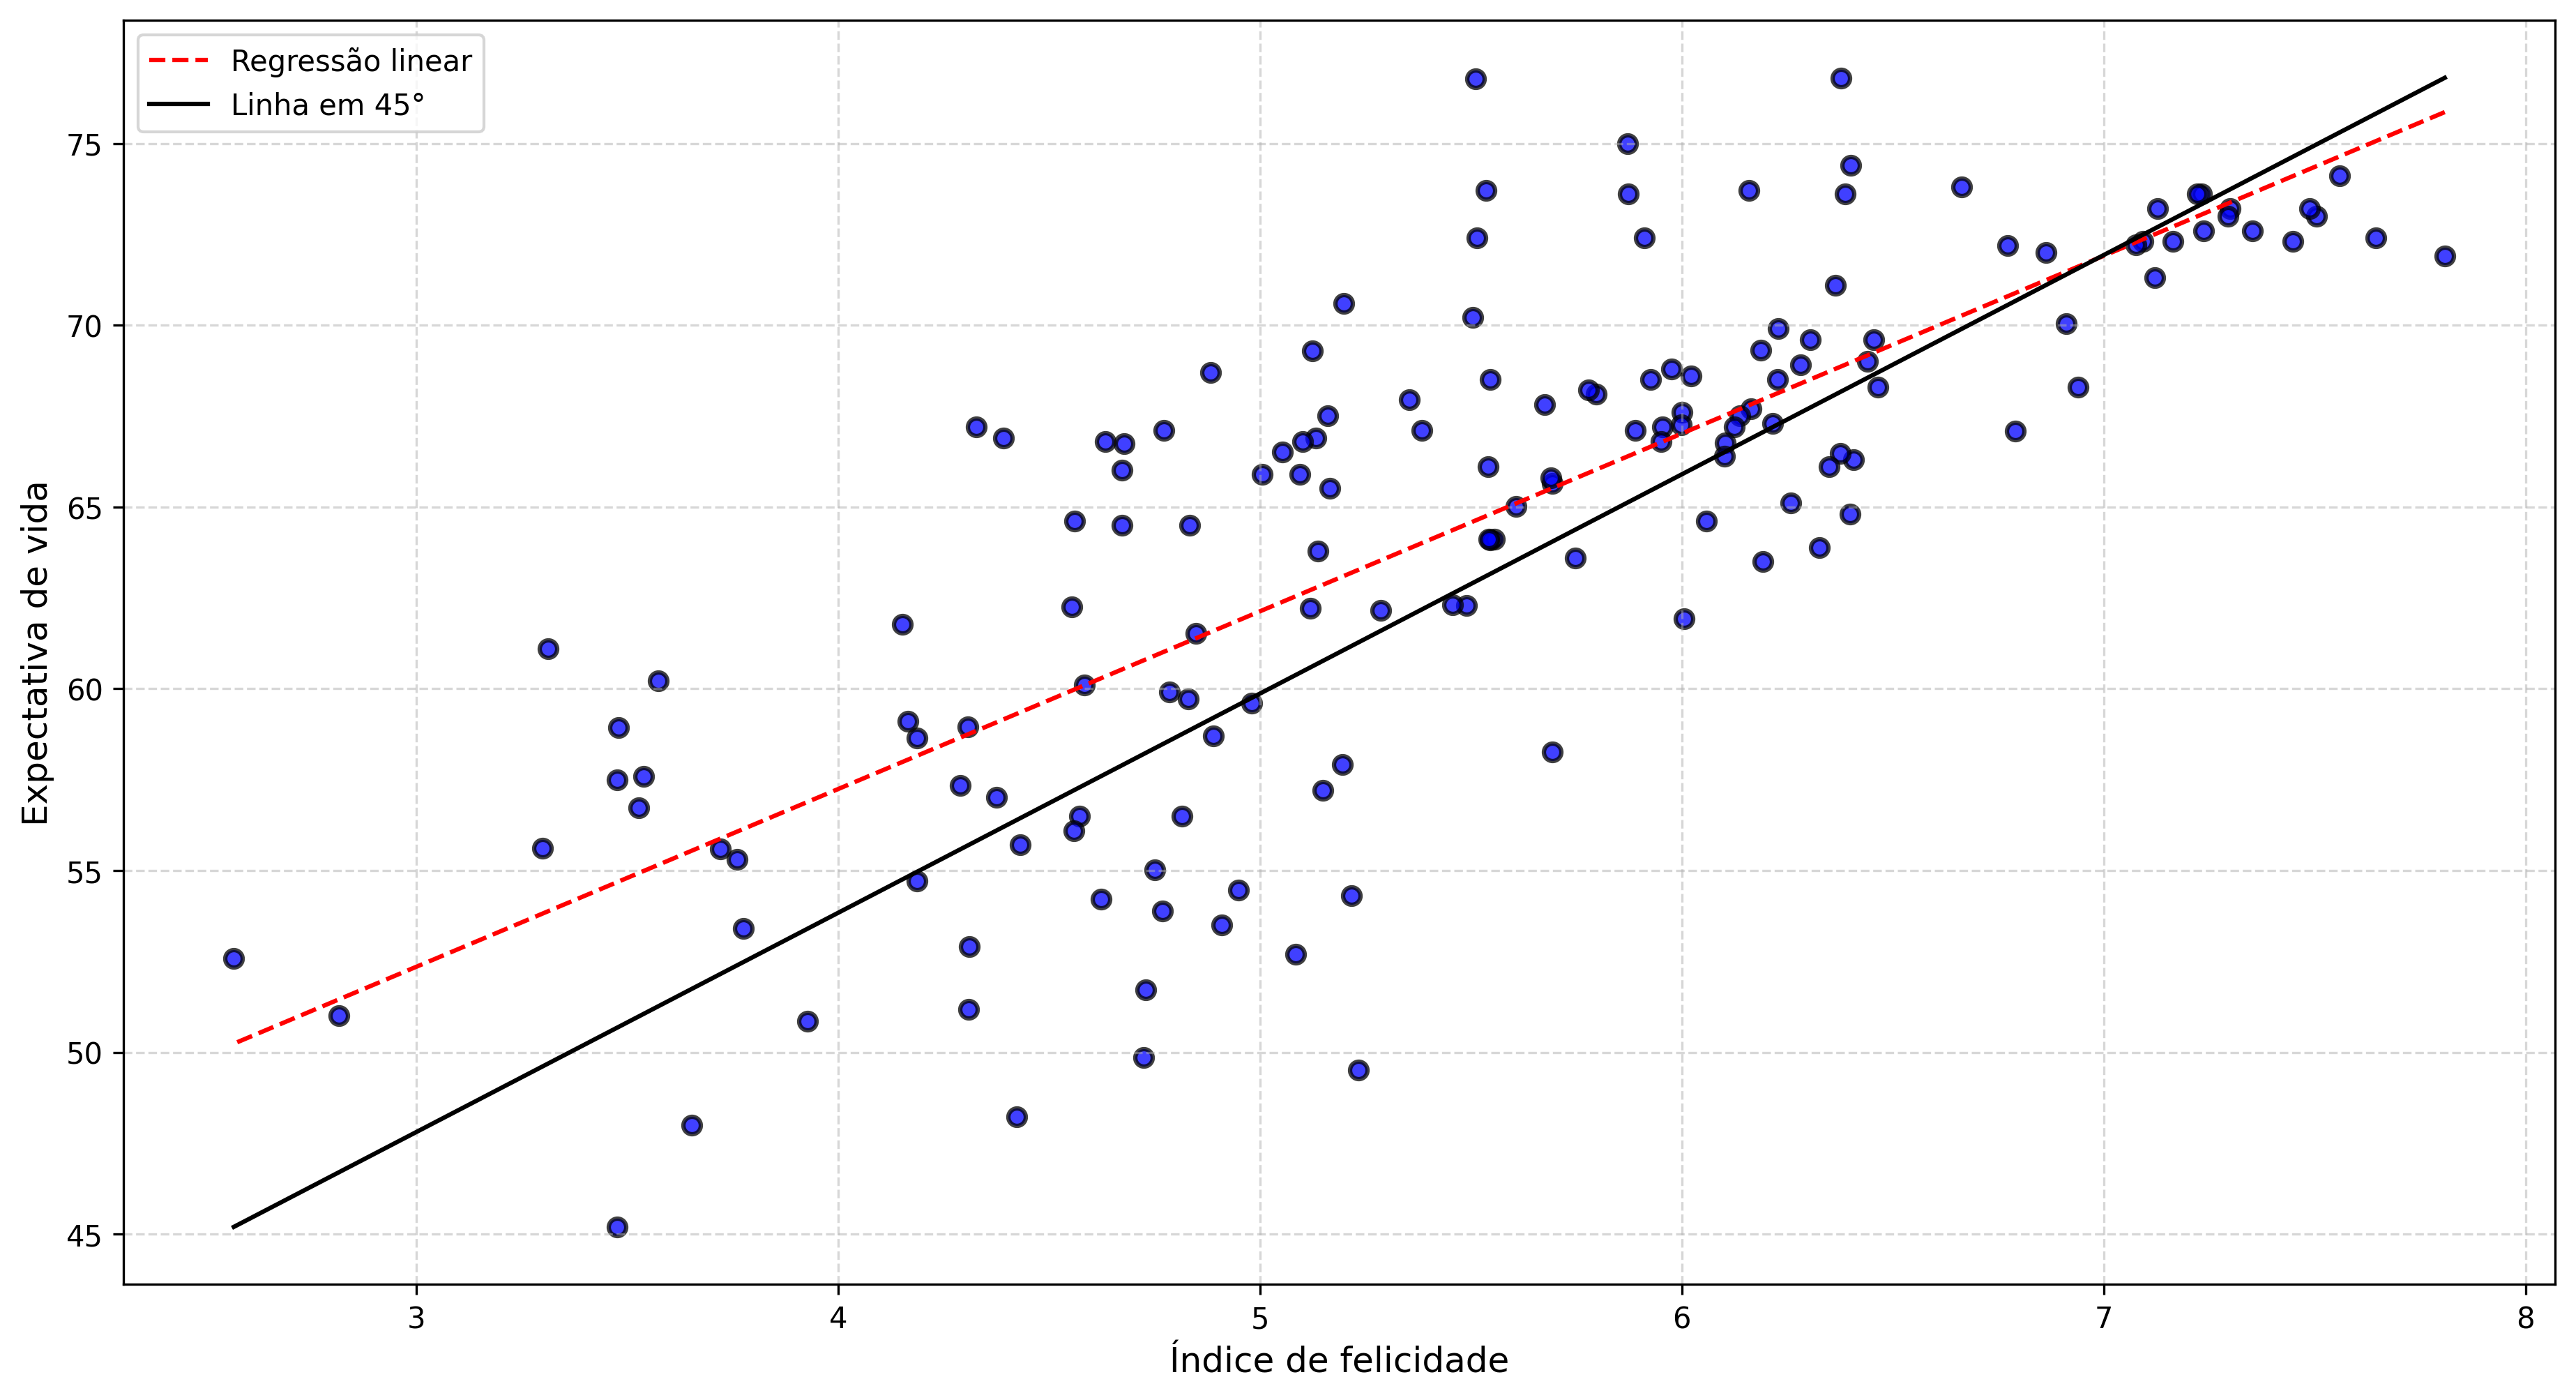
\includegraphics[scale=0.4]{figuras/happiness_world.png}
	\end{center}
	\fonte{\cite{helliwell2020}}
\end{figure}

Embora uma inferência inicial permita constatar uma correlação entre as váriavéis da equação, a criação de um modelo de previsão necessita de métodos que comprovem a correlação pressuposta. Para determinar as relações entre as variáveis dependentes e independentes de um sistema, coeficientes de correlação são calculados, gerando valores que medem e comprovam estatisticamente o grau de correspondência dos fatores estudados. Uma das métricas de correlação mais utilizadas é o coeficiente de Pearson, que mede a associação linear entre duas variáveis \cite{kirch2008}. 

Esse coeficiente de correlação pode ser definido pela Equação \ref{eq:correlacao_person}, onde $n$ é o total de amostras, $\bar{x}$ e $\bar{y}$ são as médias aritméticas de ambas as variáveis. Os valores do coeficiente de Pearson variam entre -1 e 1, de tal forma que quanto mais próximos desses extremos, melhor correlacionado estão as variáveis.

\begin{equation}
    r_{xy} = \frac{\sum_{i=1}^n (x_i - \bar{x})(y_i - \bar{y})}{\sqrt{\sum_{i=1}^n (x_i - \bar{x})^2 \sum_{i=1}^n (y_i - \bar{y})^2}}
    \label{eq:correlacao_person}
\end{equation}

A Figura \ref{fig:correlacoes} mostra alguns exemplos com gráficos de dispersão de variáveis com diferentes correlações.

\begin{figure}[H]
	\caption{\label{fig:correlacoes}Diferentes correlações entre variáveis.}
	\begin{center}
		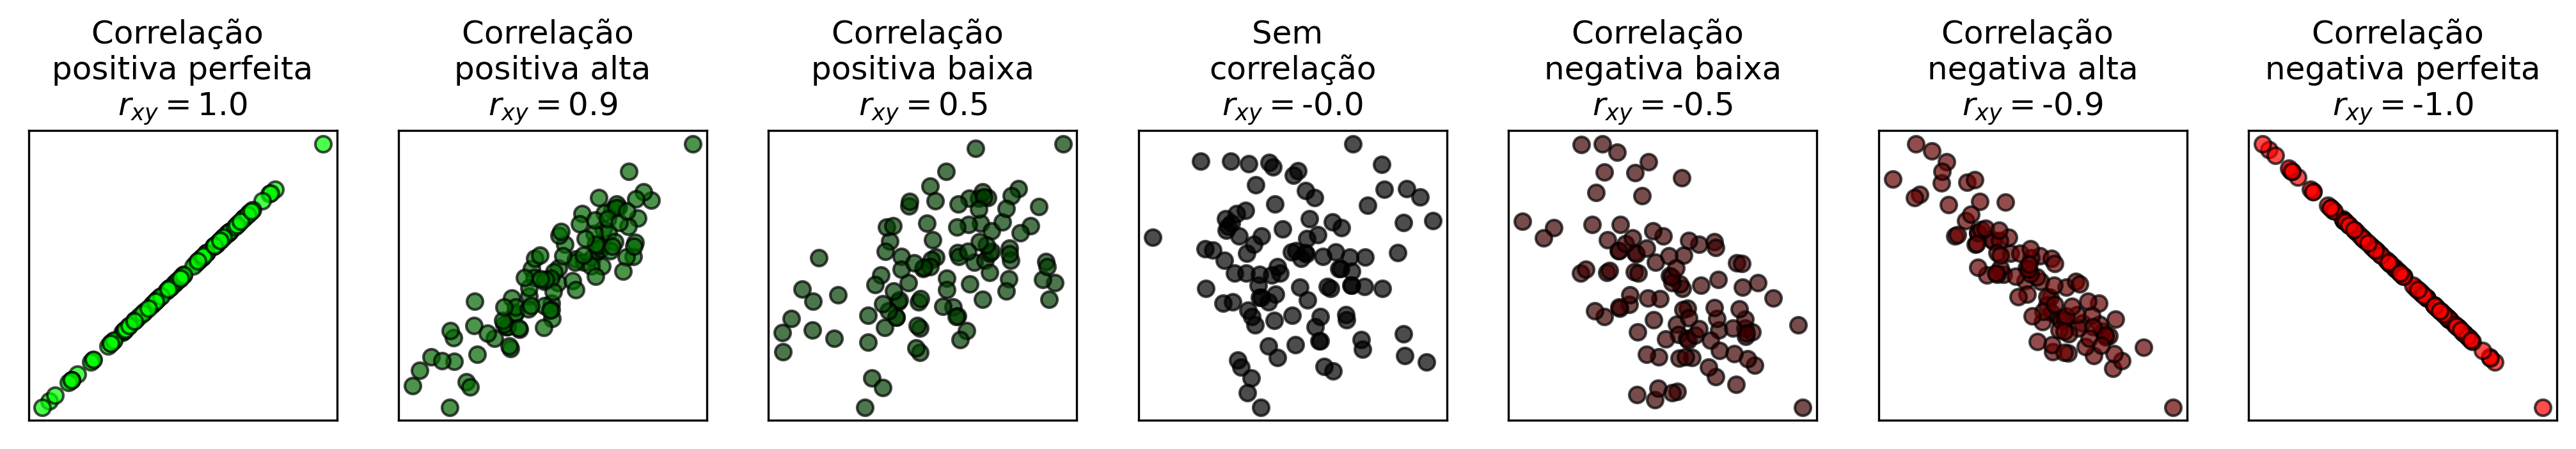
\includegraphics[scale=0.4]{figuras/correlations.png}
	\end{center}
	\fonte{\cite{helliwell2020}}
\end{figure}

Com a aplicação do método de correlação, torna-se possível estimar valores não existentes na amostra ou conjunto de dados, dando forma a uma abordagem preliminar de previsão de dados. Todavia, em casos onde a correlação entre as variáveis é baixa, a previsão de valores passa a ser menos precisa e acurada, sendo necessário outras abordagens mais robustas para realizar as previsões. Em ML, os modelos de regressão podem ser criados a partir de diversos métodos, com ajustes de parâmetros simples ou complexos que auxiliam no ajuste do modelo e seu desempenho na situação aplicada.

\section{Regressão Linear}

A regressão linear é uma técnica de análise de dados que permite estimar valores desconhecidos com base em variáveis conhecidas relacionadas. Esse modelo representa a relação entre uma variável dependente, que se deseja prever, e uma ou mais variáveis independentes através de uma equação linear \cite{aws2024}.

A aplicação da técnica é relevante devido à sua simplicidade e capacidade de fornecer previsões baseadas em uma fórmula matemática interpretável. Além disso, o método é base para implementações de algoritmos na área de ciência de dados, como aprendizado de máquina, otimizando o processamento de dados complexos e viabilizando a criação de modelos de previsão.\cite{aws2024}.

O método de regressão linear é dividido em dois grupos, sendo eles: regressão linear simples (RLS) e regressão linear múltipla (RLM). A RLS tem como objetivo estabelecer uma relação entre duas variáveis através de uma função, cuja definição é dada por:

\begin{equation}
	y_i = \alpha + \beta x_i 
\end{equation}

Onde $y_i$ é a variável alvo, enquanto $\alpha$ e $\beta$ são coeficientes calculados pela regressão, que representam o intercepto no eixo Y e a inclinação da reta, respectivamente.

A RLM, embora seja semelhante à RLS, possui múltiplas variáveis preditoras, sendo definida por:

\begin{equation}
	y_i = \alpha + \beta x_{i1} + \beta x_{i2} + ... + \beta x_{in}
\end{equation}

Onde $y_i$ é a variável alvo, $\alpha$ permanece sendo o coeficiente de intercepto do eixo Y enquanto $\beta_1$ a $\beta_n$ representam os coeficientes associados à n-ésima variável \cite{sassi2012}.

\section{Método dos quadrados ordinários}

O modelo de treinamento utilizando regressão linear consiste em  encontrar os valores apropriados para os coeficientes, determinando assim a dinâmica da função a ser estimada \cite{soczi2024}. Isso é feito usando o método dos mínimos quadrados, onde procura-se os valores que minimizam a Soma Residual dos Quadrados (RSS):

\begin{equation}
    RSS = \sum_{i=1}^{n} \left(y_i - \beta_0 - \sum_{j=1}^{p}\beta_jx_{ij}\right)
\end{equation}

onde:

\begin{itemize}
    \item $y_i$ é uma variável aleatória e representa o valor da variável resposta (variável dependente) na i-ésima observação
    \item $x_{ij}$ representa o valor da variável explicativa (variável independente, variável regressora) na i-ésima observação. Nota-se que podem existir múltiplas variáveis independentes para uma variável independente; 
    \item $\beta_{0}$ e $\beta_{j}$ são os parâmetros do modelo que serão estimados, e que definem a reta de regressão
\end{itemize}

Desse modo, a partir de um problema onde uma ou mais entradas geram amostras que resultam em uma saída, torna-se possível estimar uma função que melhor representa seu comportamento, minimzando ao máximo o valor da soma residual dos quadrados entre os pontos amostrais e a curva do modelo. 

\begin{figure}[htb]
	\caption{\label{fig:minimos_quadrados}Exemplo do método dos quadrados ordinários.}
	\begin{center}
		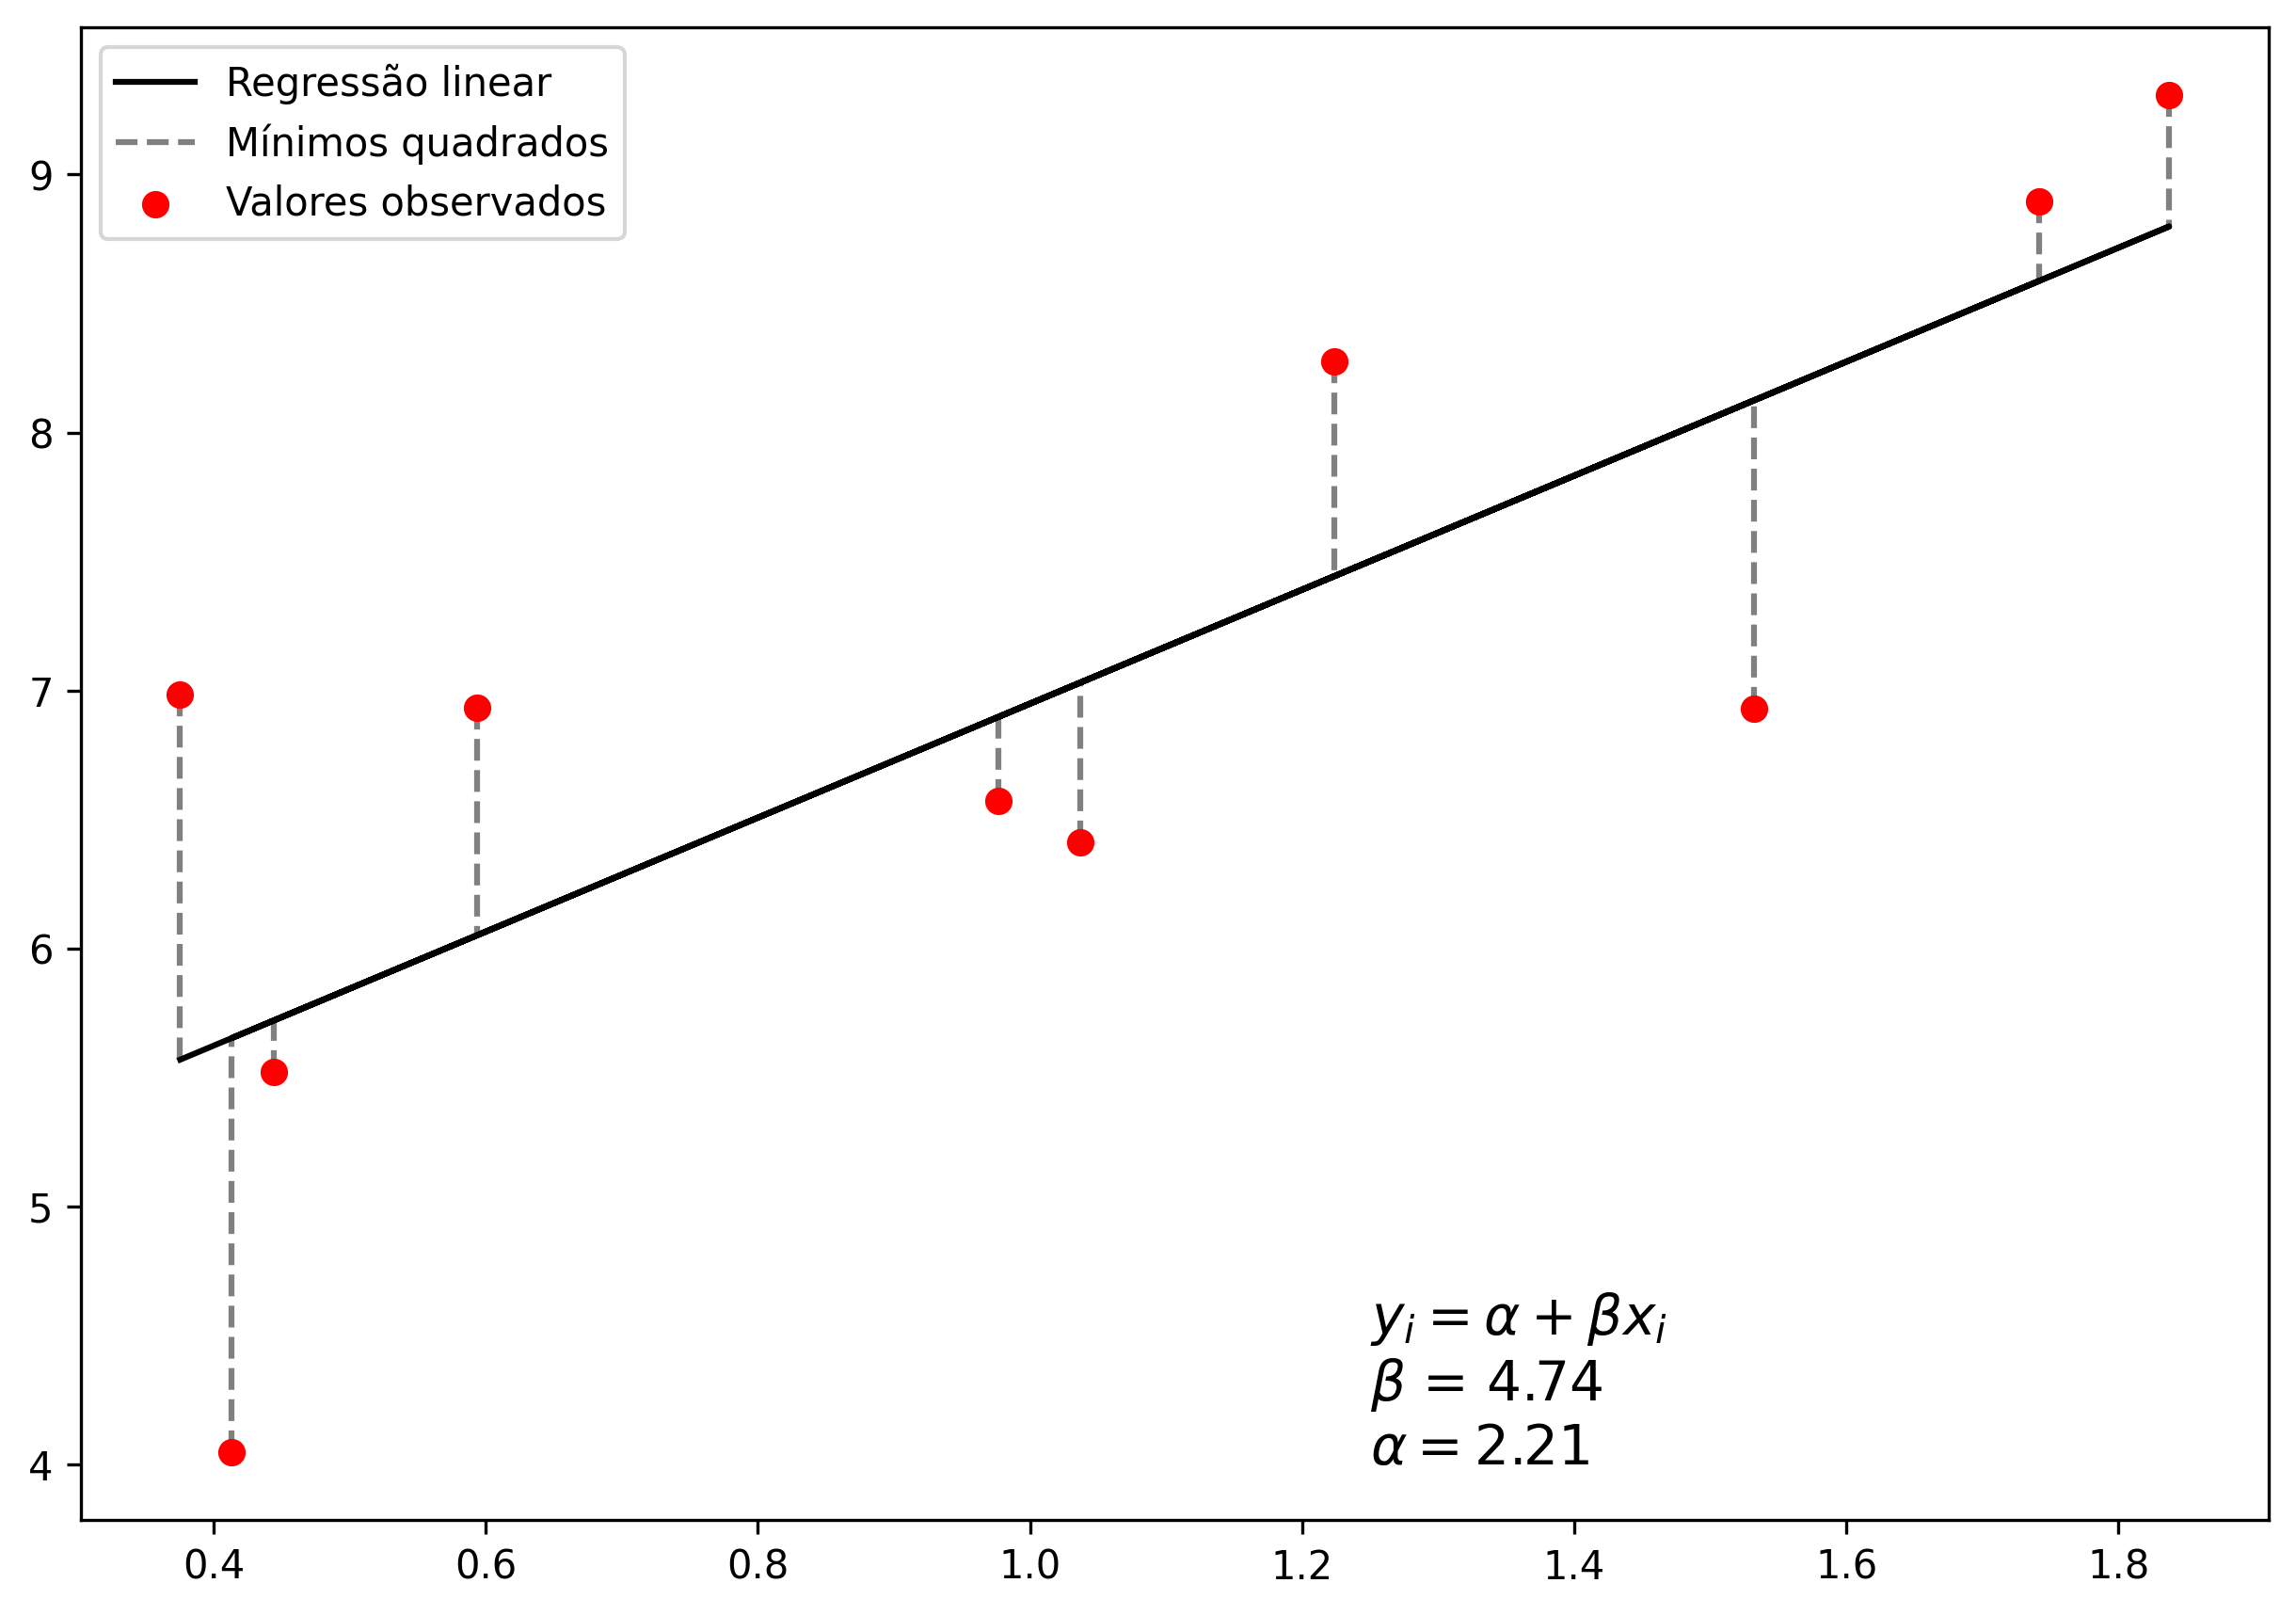
\includegraphics[scale=0.6]{figuras/min_sqr.png}
	\end{center}
	\fonte{\cite{dataat2024}}
\end{figure}

\section{Modelo Ridge}

O modelo Ridge, implementado na biblioteca \textit{scikit-learn} do Python, é uma variação da regressão linear que incorpora um termo de regularização L2 à função de custo, o que ajuda a controlar a complexidade do modelo e prevenir o sobreajuste (\textit{overfitting}). Com essa caracterísica, o método é indicado em casos onde os dados apresentam colinearidade ou onde há muitas variáveis independentes \cite{Jolly2018}.

A regressão linear padrão visa minimizar a soma dos erros quadráticos (Erro Quadrático Médio ou MSE) entre as previsões e os valores reais. No entanto, em casos onde o dataset apresenta muitos recursos ou quando os dados apresentam correlações entre as variáveis, o modelo tende a se ajustar demais aos dados de treinamento (\textit{overfitting}). A fim de contornar tal problema, o modelo Ridge adiciona um termo de penalidade à função de custo, que regula o tamanho dos coeficientes do modelo. Esse comportamento é observado na função de custo do modelo, com a adição de um hiperparâmetro $\lambda$ em relação ao modelo de regressão linear padrão.

\begin{equation}
    J(\theta) = \frac{1}{m}\sum_{i=1}^{m}\left(h_{\theta}(x^{(i)})- y^{(i)}\right)^2 + \lambda\sum_{j=1}^{n}\theta^{2}_{j}
\end{equation}

onde:

\begin{itemize}
    \item $\lambda$ é o hiperparâmetro que controla a intensidade da regularização;
    \item $\theta_{j}$ são os coeficientes (ou pesos) do modelo;
    \item Quanto maior o valor de $\lambda$, maior será a penalização para grandes coeficientes, resultando em um modelo mais simples.
\end{itemize}

Sendo assim, a inclusão do termo somado a equação de regressão linear padrão reduz a magnitude dos coeficientes, ajudando a controlar o \textit{overfitting}. Em essência, o modelo Ridge evita que o modelo aprenda padrões específicos do conjunto de treinamento que não se generalizam bem para dados novos.



